In the following, seven applications are presented to illustrate the versatility of Bioptim and to give a practical overview on how to use its main features.
The performances and the Github links of each OCP are summarized in Tab.~\ref{tab:Perfs_and_detailed_implementations_of_each_example}.


\subsection{Muscle activation driven pointing task}
%
In this first example, the goal was to achieve a muscle activation driven pointing task using a 2-DoF arm model with six muscle elements. 
In addition to muscle-induced torques, pure joint torques were added to compensate for the model weaknesses.
The main term (highest weight) of the objective function (Eq.~\ref{eq:cost_pointing}) is a Mayer objective, corresponding to the pointing tasks at the final node, to superimpose two markers, the first one ($\mathbf{m_u}$) fixed in the ulna system of coordinates and the second one ($\mathbf{m^*_s}$) fixed in the scene.
The three Lagrange terms  were added for control (muscle activation $\bf{a}$ and joint torques $\boldsymbol{\tau}$) and state ($\bf{x}$) regularization:
\[
\begin{aligned}
	\mathcal{J} = 	&~\omega_1~\underbrace{\|\mathbf{m_u}(T)-\mathbf{m^*_s}\|^2}_{\mathtt{TRACK\_MARKERS}}~\\
	&\int_{t=0}^T\underbrace{\|\bf{a}\|^2}_{\mathtt{MIN\_ACTIVATION}}~
	+\underbrace{\|\boldsymbol\tau\|^2}_{\mathtt{MIN\_TORQUE}}~
	+\underbrace{\|\bf{x}\|^2}_{\mathtt{MIN\_STATE}}~ dt,
\end{aligned}
\addtag
\label{eq:cost_pointing}
\]

\noindent where $T\!=\!\SI{2}{\second}$ is the duration of the motion, and $\omega_1\!=\!1e5$.
The problem was discretized using 50~shooting nodes with a 5-steps Runge-Kutta-4 (RK4) integration in-between.
The problem was solved using \ipopt (with exact Hessian computations) and \acados (with a Gauss-Newton approximation of the Hessian) resulting in two very close solutions.
\acados was about 50 times faster than \ipopt and was better at enforcing the continuity constraints (as shown by the single shooting error in Tab.~\ref{tab:Perfs_and_detailed_implementations_of_each_example}).
\ipopt however ended up with a smaller optimized objective (20.8 \textit{vs} 23.2), leading to a more optimal solution than \acados. 
Superimposed snapshots of the optimal motion found with \acados are displayed in Fig.~\ref{fig:snapshots_activation_driven_pointing}.
It is worth mentioning that for the purpose of this illustration, no constraint was given on the shoulder range of motion to ensure physiological muscle trajectories. 


\subsection{Quaternion base twisting somersault}
In this example of acrobatic sports biomechanics, the goal was to maximize the twist rotation ($\phi$) of a 8-DoF model in a backward somersault.
The model was composed of a 6-DoF root segment and two 1-DoF torque actuated shoulder joints.
Two different numerical description of the root segment rotations were used (Euler angles and quaternions).
The objective function was as follows:

\begin{eqnarray}\label{eq:ocp_Trampo}
\mathcal{J} = \omega_1 \underbrace{\int_0^T \dot{\phi}~dt}_{\mathtt{MIN\_TWIST}}  +~\omega_2 \underbrace{\int_0^T \sum_{i=1}^{2}~\tau_{i}^2~dt}_{\mathtt{MIN\_ TORQUE}},
\end{eqnarray}
with $\omega_1 = -1$ (resulting in the maximization of the first term) and $\omega_2 = 1\times 10^{-6}$, T the duration of the movement and $\tau_{i}$ the torque control input of the $i^{th}$ arm DoF.
The first term of the objective function (Eq.~\ref{eq:ocp_Trampo}) corresponds to maximizing the twist velocity and the second term serves as control regularization.


The movement lasted for approximately 1 second and was discretized with 80 shooting nodes.
The solutions for both models were \comment{similar}{ce n'est pas vraiment le cas, commenter} (Fig.~\ref{fig:snapshots_quaternion_base_twisting_somersault}) highlighting the equivalence of the two rotation representations.
Euler angles have the advantage to be easily interpretable, but they suffer from the loss of a DoF at the Gimbal lock (leading to numerical instabilities).
The use of a quaternion-based representation is tackles this numerical stability issue when a joint is free to rotate on a three-dimensional range of motion.
Quaternion's integration must be handled with care~\cite{bailly2020optimal}, which was taken care of in \textit{bioptim}.


\begin{figure*}[t!]
\centering
\includegraphics[width=\textwidth]{figures/Euler_Bioptim_MaxVrille_dos.png}\\
\vspace*{0.5em}
\includegraphics[width=\textwidth]{figures/Quat_Bioptim_MaxVrille_dos.png}
\caption{Snapshots of a maximally twisting somersault driven by shoulder torque actuators and a free base expressed by Euler angles (top) or quaternions (bottom).}
\label{fig:snapshots_quaternion_base_twisting_somersault}
\end{figure*}


% \begin{table}[h!]
% \caption{\small Objective terms of quaternion base maximally twisting somersault}
% \label{tab:Quaternion_base_twisting_somersault}
% \centering
% \begin{tabular}{c c c c}
% \toprule 
% & Type & Function & Weight \\ 
% \midrule
% $\#1$ & Lagrange & MINIMIZE\_TWIST & $-1e1$ \\ 
% \midrule
% $\#2$ & Lagrange & MINIMIZE\_ TORQUE & $1e-6$ \\ 
% \bottomrule
% \end{tabular}
% \end{table}















\subsection{Multiphase torque driven walking cycle}
This walking example is presented to introduce \textit{bioptim}'s ability to deal with gait biomechanics as a multiphase problem with contact forces.
The goal was to estimate muscles activation by tracking markers trajectories, ground reaction forces and moments (Equations.~\ref{eq:ocp_markers}, ~\ref{eq:ocp_forces} and ~\ref{eq:ocp_moments}, respectively). 
The model was driven by muscle activation. 
To predict muscle activity, the objective function consisted in finding the least squared muscle activations $a_{i}$ (Equations.~\ref{eq:ocp_muscles}). 
Pure residual torques were also added to compensate potential underactuation from the model weaknesses and penalized as shown in equation ~\ref{eq:ocp_torques}.\\
The gait cycle was defined from the first heel strike to the end of the swing phase using a simplified 3D one-leg model with 12 DoFs and 17 muscles (pelvis + right lower limb). 
Based on experimental force plateform data and markers position, the stance was divided into three phases (heel, flatfoot and forefoot contacts) of fixed duration (0.05, 0.355 and 0.16s), to follow the natural rolling movement of the foot from heel strike to toe off.
The swing phase lasted 0.38 s. 
The interaction between the ground and the foot was modelled using a 4-contact points model located at the heel and the forefoot (first, fifth metatarsi and hallux).

The complete cycle was discretized in 90 intervals and the objective functions are written as follow :\\

%\[ 
%\resizebox{0.9\columnwidth}{!}{$ 
%\begin{aligned}
%\mathcal{J} = &\int_{t=0}^{T}\underbrace{\omega_1(\|m_p - m_m\|^{2})}_{\mathtt{TRACK\_MARKERS}}~ 
%+ ~ \underbrace{\omega_2(\|f_p - f_c\|^{2})}_{\mathtt{TRACK\_FORCES}}\\
%&+ ~ \underbrace{\omega_3(\|tau^f_p - tau^f_m\|^{2})}_{\mathtt{TRACK\_MOMENTS}}~
%\mathcal{J} = &\int_{t=0}^{T}\underbrace{\omega_1(\|m_p - m^*_m\|^{2})}_{\mathtt{TRACK\_MARKERS}}~ 
%+ ~ \underbrace{\omega_2(\|f_p - f^*_c\|^{2})}_{\mathtt{TRACK\_FORCES}}\\
%&+ ~ \underbrace{\omega_3(\|tau^f_p - tau^{f*}_m\|^{2})}_{\mathtt{TRACK\_MOMENTS}}~
%+ ~ \underbrace{\omega_4\|a\|^2}_{\mathtt{MIN\_ACTIVATION}}~dt, 
%\end{aligned}  
%$}  
%$}
%\addtag  
%\label{eq:ocp_walk}  
%\]

\begin{eqnarray}
\label{eq:ocp_markers}
\mathcal{J} = \sum_{i=1}^{N_i}\Bigg(\underbrace{\omega_1(\|m_p - m_m\|^{2})}_{\mathtt{TRACK\_MARKERS}}
\end{eqnarray}
\begin{eqnarray}
\label{eq:ocp_forces}
+ \underbrace{\omega_2(\|\sum_{c=1}^{N_c}F_p - F_m\|^{2})}_{\mathtt{TRACK\_FORCES}}
\end{eqnarray}
\begin{eqnarray}
\label{eq:ocp_moments}
+ \underbrace{\omega_3(\|\sum_{c=1}^{N_c}M_p - M_m\|^{2})}_{\mathtt{TRACK\_MOMENTS}}
\end{eqnarray}
\begin{eqnarray}
\label{eq:ocp_muscles}
+ \underbrace{\omega_4\int_0^T \sum_{i=1}^{N_i}~a_{i}^2~dt}_{\mathtt{MINIMIZE\_ ACTIVATION}})  
\end{eqnarray}
\begin{eqnarray}
\label{eq:ocp_torques}
+ \underbrace{\omega_5\int_0^T \sum_{i=1}^{2}~\tau_{i}^2~dt}_{\mathtt{MINIMIZE\_ TORQUE}}\bigg)
 \end{eqnarray}

where $\omega_{i}$ are the weighting factors ($\omega_1$=1e5, $\omega_2$=0.1, $\omega_3$=0.1, $\omega_4$=10, $\omega_5$=1), $T$ is the the duration, $N_i$ and $N_c$ are the number of time frames and contact points of the current phase. The indices $_p$ and $_m$ stand for predicted and measured data.\\

Non-slipping ($\mathtt{NON\_SLIPPING}$) and unilateral contact force ($\mathtt{CONTACT\_FORCE}$) constraints prevented the foot from slipping and pulling from the ground. 
In between phases, the use of the $\mathtt{IMPACT}$ state transition allowed to represent the gain or loss of contact(s) in the dynamics (e.g., swing phase to heel strike [thesis Felis - articles?]) \\

Fig.~\ref{fig:snapshots_multiphase_walking_cycle} shows the leg movements during the walking cycle. The mean tracking error on markers trajectories was 0.027 m (mean error on pelvic and foot markers was 0.0075 m and 0.0147 m, respectively). 
Concerning ground reaction forces tracking, the mean error was 4.85 N with an average $R^2$ at 0.9. 
Gluteal muscles were only activated during the stance phase and especially during the early flatfoot phase for the gluteus maximus with a maximal activation of 0.2. 
For the thigh muscles, the semimembranous, semitendinous and biceps femoris were activated during the early stance phase and terminal swing (maximal activation of 0.3, 0.4 and 0.4, respectively). 
The knee extensors, vastus lateralis, medialis and intermedius followed the same pattern and were mainly activated during the flatfoot phase. 
However, maximal activation of the rectus femoris appeared at early forefoot phase and early swing. Leg muscles were highly activated (saturation of gastocnemius lateralis and medialis) at the end of the stance and the early swing phase. 

\begin{figure*}[t!]
\centering
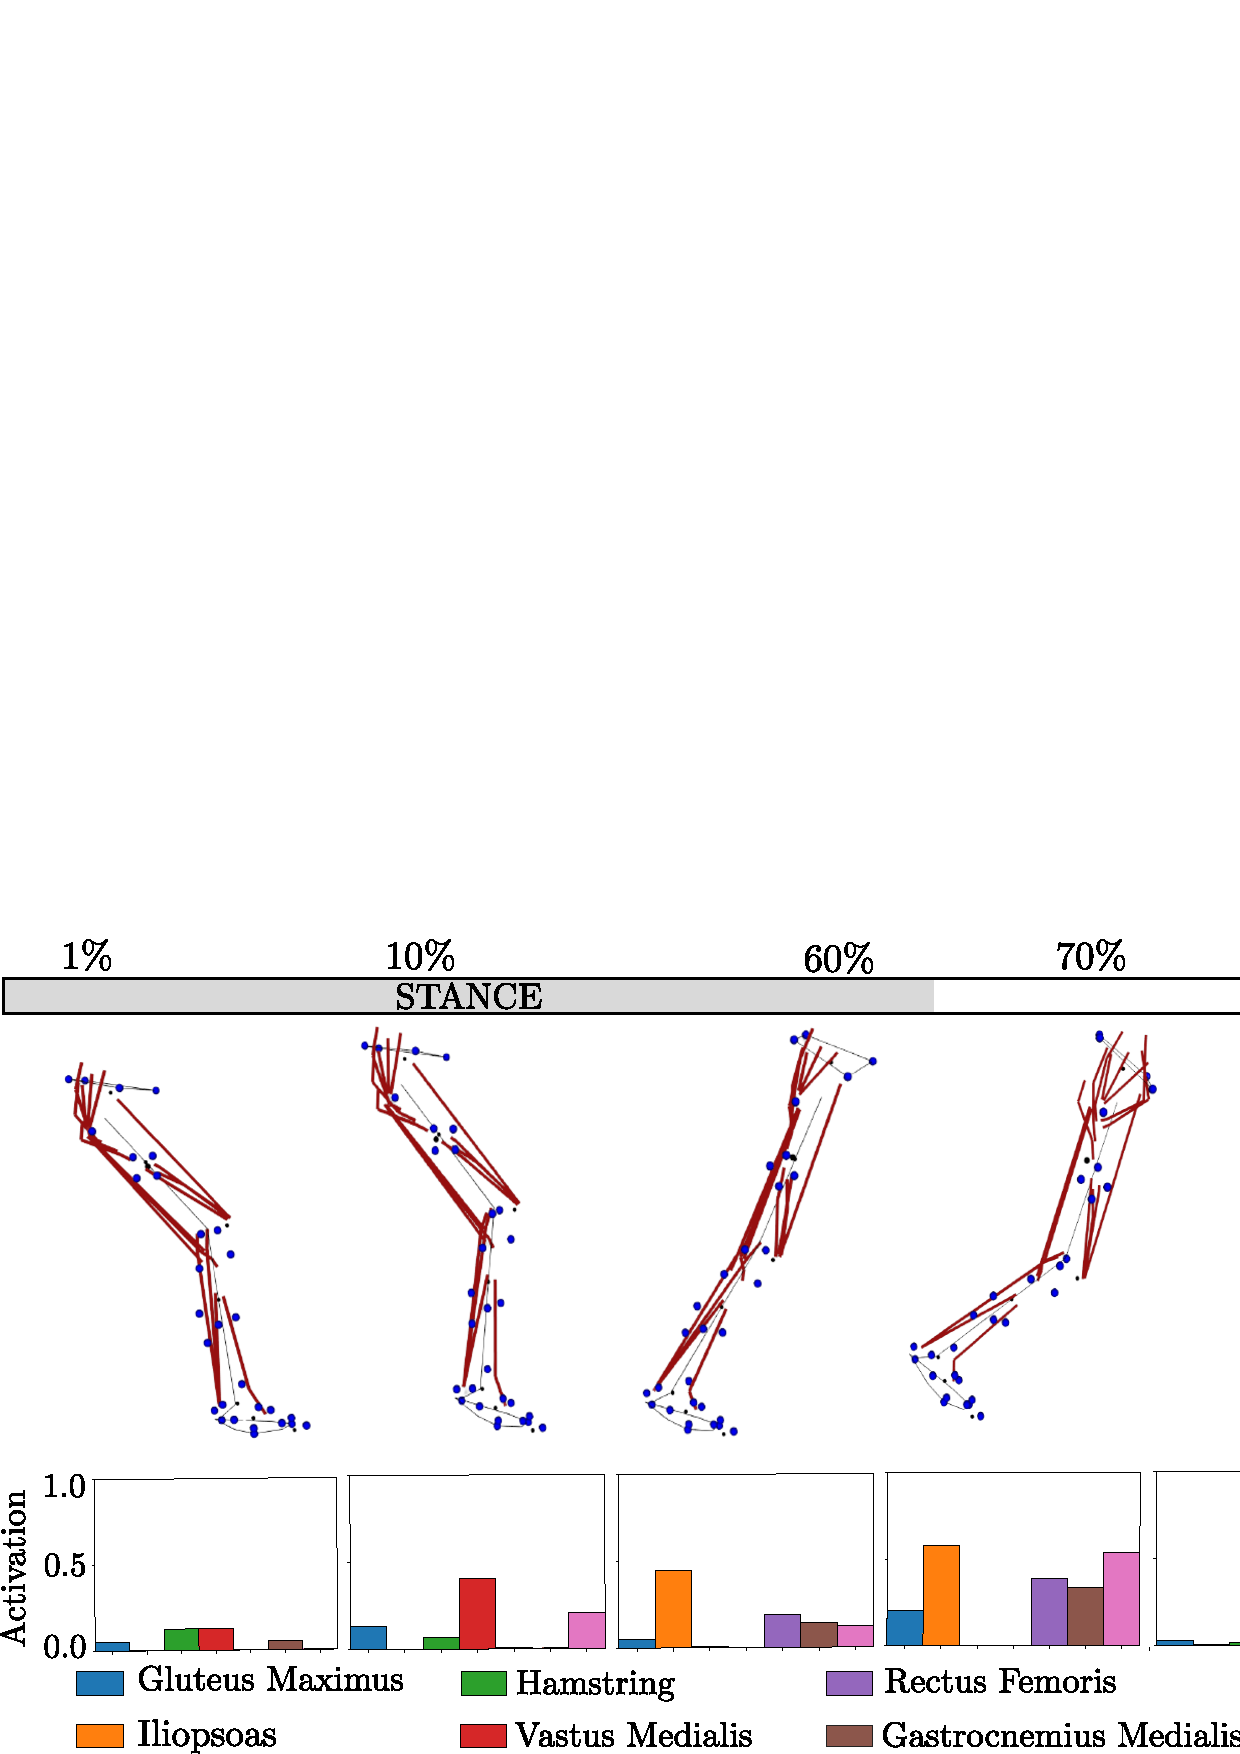
\includegraphics[width=\textwidth]{figures/multiphase_walking_cycle.png}\\
\caption{Snapshots of a walking gait cycle driven by muscles activation.}
\label{fig:snapshots_multiphase_walking_cycle}
\end{figure*}

%\begin{table}[h!]
%\caption{\small Objective terms of the Multiphase torque driven walking cycle }
%\label{tab:Multiphase_torque_driven_walking_cycle}
%\centering
%\begin{tabular}{c c c c}
%\toprule 
%& Type & Function & Weight \\ 
%\midrule
%$\#1$ & Lagrange & TRACK\_ STATE & $1e5$ \\ 
%\midrule
%$\#2$ & Lagrange & MINIMIZE\_ TORQUE\_ DERIVATIVE & $1e-2$ \\ 
%\midrule
%$\#3$ & Lagrange & TRACK\_ GRF & $1e-2$ \\ 
%\midrule
%$\#4$ & Lagrange & TRACK\_ MOMENTS & $1e-1$ \\
%\bottomrule
%\end{tabular}
%\end{table}


%
\begin{table*}[t!]
\caption{\small Overview of computational results for the different OCPs cases and links to detailed implementations. $^\star$ stands for free time OCP, otherwise it is fixed.}
\label{tab:Perfs_and_detailed_implementations_of_each_example}
\centering
\begin{tabular}{c l rl rl rl}
\cmidrule[\heavyrulewidth](lr){2-8}
& & \multicolumn{2}{l}{Activation-driven pointing} & \multicolumn{2}{l}{Ex\# 2} & \multicolumn{2}{l}{Ex\# 3} \\
\cmidrule[\heavyrulewidth](lr){3-4}
\cmidrule[\heavyrulewidth](lr){5-6}
\cmidrule[\heavyrulewidth](lr){7-8}

\mymultirow{4}{Setup} & \# states $\xt$            & \multicolumn{2}{c}{2}  & --    & --     & --    & --\\
                      & \# control $\ut$           & \multicolumn{2}{c}{8}  & --    & --     & --    & --\\
                      & \# shooting nodes          & \multicolumn{2}{c}{51} & --    & --     & --    & --\\
                      & OCP duration (s)           & \multicolumn{2}{c}{2}  & --    & --     & --    & --\\
                      &                            & IPOpt  & ACADOS        & IPOpt & ACADOS & IPOpt & ACADOS\\
\mymultirow{3}{Solve} & \# NLP iterations          & 27     & 21            & --    & --     & --    & --\\
                      & Optimized cost             & 6959.3 & 427.5         & --    & --     & --    & --\\
                      & Time to convergence (s)    & 9.9    & 0.19          & --    & --     & --    & --\\
%Example & Link & IPOPT & ACADOS \\ 
%\midrule
%Muscle activation driven pointing task & \href{https://github.com/pyomeca/BiorbdOptim/blob/master/examples/muscle_driven_ocp/static_arm.py}{$\star$} & $10.10$ & $0.2018$  \\ 
%\midrule
%$\bullet$ & $\bullet$ & $\bullet$ & $\bullet$ \\ 
\cmidrule[\heavyrulewidth](lr){2-8}
\end{tabular}
\end{table*}
%







